\documentclass{article}
\usepackage{graphicx} % Required for inserting images
\usepackage[utf8]{inputenc}
\usepackage{polski}
\usepackage[dvipsnames]{xcolor}
\usepackage{indentfirst}
\usepackage{multicol}
\usepackage{geometry}
\usepackage{titlesec}
\usepackage[colorlinks=true, linkcolor=gray, urlcolor=blue, citecolor=green]{hyperref}
\usepackage{makecell}
\usepackage{float}
\usepackage[polish]{babel}
\usepackage[T1]{fontenc}
\usepackage[justification=centering]{caption}
\usepackage[utf8]{inputenc} 
\usepackage{subfig}


\usepackage{mwe} % for 'example-image'
\usepackage{newfloat}
\DeclareFloatingEnvironment{graph}
\addto\captionspolish{%
  \renewcommand{\graphname}{Wykres}%
  \renewcommand{\figurename}{Zdjęcie}%
  \renewcommand{\tablename}{Tabela}%
}


\begin{document}

\begin{titlepage}
    \begin{center}
        \vspace*{1cm}
            
        \Huge
        \textbf{Sprawozdanie z laboratorium 4}
            
        \vspace{0.5cm}
        \LARGE
        Profibus 
            
        \vspace{1.5cm}
            
        \textbf{Łukasz Janusz\\Marek Generowicz}

        \normalsize      
        \textcolor{gray}{17.03.2025}
        \vfill
        \begin{figure}[hb]
            \centering
            
\includegraphics[width=0.5\textwidth]{media/Logo_AGH.jpg}
        \end{figure}   
    \end{center}
\end{titlepage}

\section{Wstęp}
Na laboratorium należało zapoznać się z komunikacją po sieci Profibus pomiędzy sterownikiem S7-1200 a oddaloną wyspą pomiarową Simatic ET 200SP. Komunikacja ta stosowana jest w przemyśle do komunikacji pomiędzy urządzeniami pomiarowymi a sterownikami PLC zazwyczaj znajdującymi się w szafie sterowniczej. Zasadniczą zaletą jest możliwość połączenia urządzenia pomiarowego z PLC na duże odległości, nawet do 1200 metrów. Dodatkowo do jednej sieci Profibus można podłączyć maksymalnie 32 urządzenia.

\section{Opis Stanowiska}
Na stanowisku laboratoryjnym (Zdjęcie \ref{fig:stanowisko}) znajdował się sterownik S7-1200 marki Siemens połączony z modułem Profibus CM 1243-5 (DP-Master). Osobną część stanowiła wyspa pomiarowa wyposażona w moduł wejść/wyjść oddalonych ET 200SP, moduł wejść temperaturowych 4xRTD/TC oraz moduł wyjść dyskretnych DQ 8x 24V DC/0.5A. Wyspa pomiarowa była połączona z sterownikiem za pomocą kabla Profibus. urządzenia były zasilane zasilaczem ET 200SP. Do pomiarów wykorzystano czujnik temperatury Pt100 oraz termoparę. Fizycznymi elementami informacyjnymi były dwie diody LED.  

\begin{figure}[H]
    \centering
    \includegraphics[width=0.92\textwidth]{media/Cale_stanowisko.jpg}
    \caption{Stanowisko laboratoryjne}
    \label{fig:stanowisko}
\end{figure}

\section{Konfiguracja sterownika}

Konfigurację rozpoczęto od dodania sterownika \textit{SIMATIC S7-1200} do projektu w programie \textit{Tia portal V19}. Następnie dodano moduł Profibus w katalogu \textit{Hardware catalog}. Potwierdzeniem poprawnego dodania modułów jest poniższa konfiguracja sprzętowa (Zdjęcie \ref{fig:konfiguracja}).

\begin{figure}[H]
    \centering
    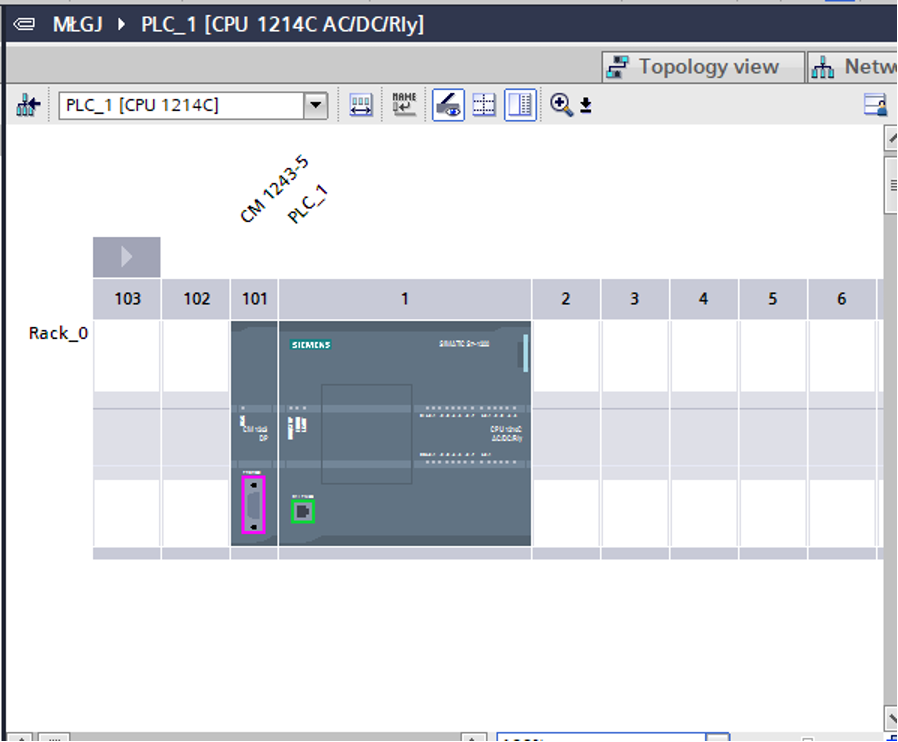
\includegraphics[width=1\textwidth]{media/4PLCKonfiguracja.png}
    \caption{Konfiguracja sprzętowa}
    \label{fig:konfiguracja}
\end{figure}

Kolejno ustawiono adres sieciowy sterownika na \textbf{10.10.4.10} oraz zmieniono wartość maski na \textbf{255.255.0.0}.

Następnym krokiem było dodanie modułów z wyspy pomiarowej do projektu. Zaczęto od modułu I/O oddalonych ET 200SP, który został dodany poprzez przeciągnięcie go z \textit{Hardware catalog} do \textit{Network view}. W zakładce \textit{Properties} modułu \textit{Slave} wartość Profibus address została ustawiona na 3, ponieważ taki sam adres był ustawiony na fizycznym module. Po tej operacji moduły \textit{PLC\_1} oraz \textit{Slave\_1} zostały połączone kablem Profibus (Zdjęcie \ref{fig:polaczenie}). 

\begin{figure}[H]
    \centering
    \includegraphics[width=1\textwidth]{media/3Połączenie.png}
    \caption{Połączenie modułów}
    \label{fig:polaczenie}
\end{figure}

W ustawieniach sieciowych połączenia prędkość została ustawiona na 1.5 Mb/s, a profil na Modbus DP. Pozostałe parametry dostępne w menu \textit{Bus parameters} zostały ustawione automatycznie i nie były modyfikowane.

Kolejnym krokiem było konfigurowanie urządzenia \textit{Slave\_1}. Po dwukrotnym kliknięciu na jego ikonkę otworzyła się zakładka \textit{Device view} wraz ze szczegółami wyspy pomiarowej. Do wyspy dodany został moduł wejść temperaturowych \textit{AI 4xRTD/TC 2-,3-,4-wire HF} oraz moduł wyjść dyskretnych \textit{DQ 8x 24V DC/0.5A}. Firmware pierwszego z modułów został ustawiony na 2.0. W podobny sposób dodano moduł końcowy \textit{Server module}. Ostatecznie urządzenie \textit{Slave\_1} prezentowało się następująco: (Zdjęcie \ref{fig:slave1}).

\begin{figure}[H]
    \centering
    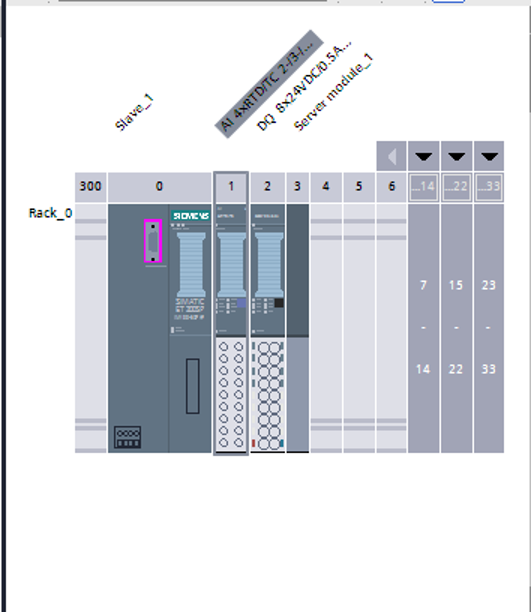
\includegraphics[width=0.723\textwidth]{media/1Wyspa_profibus.png}
    \caption{Konfiguracja urządzenia Slave\_1}
    \label{fig:slave1}    
\end{figure}

\section{Konfiguracja modułu pomiarowego}

\end{document}
